%Kinwalker_Bac - Progress report
\documentclass{beamer}
\usepackage{graphicx}
\usepackage{amsmath,amsfonts,amssymb}
%exclude navigation symbols
\beamertemplatenavigationsymbolsempty
\usetheme[compress]{Dresden}
\usecolortheme{seagull}
\usefonttheme{structurebold}
\expandafter\def\expandafter\insertshorttitle\expandafter{\insertshorttitle\hfill\insertframenumber\,/\,\inserttotalframenumber}

\usepackage{amsmath} % write contitions within the equations

\title{In silico analysis of RNA co-transcriptional folding }

\author[Mario Koestl]{Mario Koestl}
\institute[TBI]{Institute for Theoretical Chemistry\\ University of Vienna}
\date{\today}
\subject{}
\keywords{}
%\newcommand{\TODO}[1]{{\color{red} #1}}
\begin{document}
\frame{
  \titlepage
}

\frame{
\frametitle{Motivation}
\begin{itemize}
\item Are evolutionary conserved folding pathways present in related RNA sequences?
\item Is it possible to predict such pathways by using kinetic heuristics like \texttt{Kinwalker}?
\item How should the \texttt{Kinwalker} parameters be fine-tuned to better reflect reality?
\end{itemize}
}


\frame{
\frametitle{RNA basics}
\begin{itemize}
\item RNA $\Rightarrow$ nucleotid subunits
\item Nucleotid $\Rightarrow$ nucleobase, ribose and phosphat group
\item Nucleobase $\Rightarrow$ Adenin, Cytosin, Guanin, Uracil
\item RNA is directional molecule
\item RNA (5'$\Rightarrow$ 3') is exact copy of DNA leading strand (5' $\Rightarrow$ 3')
\end{itemize}

\begin{figure}
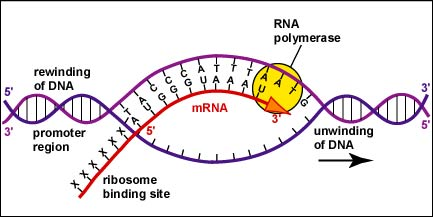
\includegraphics[scale=0.4]{pictures/transcription.jpg}
\end{figure}

}

%For better understanding I will start with the basics of RNA molecules and their co-transcriptional folding, because everything inside this thesis is related to RNAs.

%RNA is a polymer molecule consisting of smaller subunits called nucleotids
%A nucleotide is composed of a nucleobase, a ribose
%monosaccharid and a phosphate group. The nucleobase can either be an
%Adenin(A), Cytosin(C), Uracil(U) or a Guanin(G). Nucleotides are linked
%together by covalent bonds, resulting in a sugar-phosphate backbone.
%
%
%RNAs are formed during transcription, executed by different RNA polymerases. In detail, the DNA template strand (3'-> 5') is read by a RNA polymerase and a new single RNA strand is formed, with complementary bases.
%The newly formed strand (5'-> 3') is now an exact copy of the DNA leading strand (5' -> 3'). 
%

\frame{
\frametitle{Co-transcriptional folding}
\begin{itemize}
\item RNA refolding during transcription
\item {\bf Co-transcripitonal folding trajectory}: directed list of all created structures
\item Computing such trajectories is extremely difficult
\item Heuristic approach via \texttt{Kinwalker}
\item Secondary structure prediction during transcription
\end{itemize}
\begin{figure}
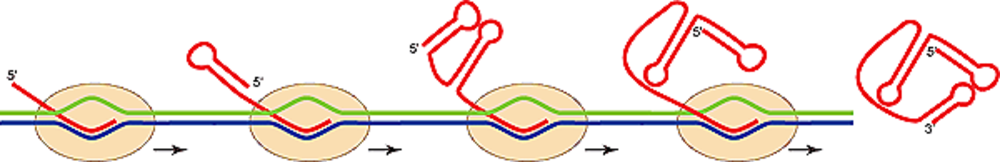
\includegraphics[scale=0.5]{pictures/coTransFolding.pdf}
\end{figure}

}

%The next basic stuff I would like to explain is the event of RNA co-transcriptional folding
%During transcription the new RNA strand is created starting with the 5' end, therefore RNA folding can occur during transcription at the sequence between the already transcribed 5' end and the transcription bubble.
%Such refoldings lead to different structures, and the directed list of all these structures is called a co-transcriptional folding trajectory.

%Computing such trajectories is extremely difficult and thus only a handful of programs exist which allow for an efficient prediction. One of them is the program
%Kinwalker. Kinwalker is a heuristic that deterministically tries to predict RNA folding kinetics.
%With Kinwalker it is possible to predict the list of all emerging secondary structures for RNA chains during transcription.
%


\frame{
\frametitle{Kinwalker}
{\bf Parameters:} \texttt{--transcription rate}, \texttt{--pathfinding algorithm},\texttt{--maxKeep, \texttt{--dangle option}}

{\bf dangling base-pairs}
\begin{itemize}
\item stacking an unpaired base to adjacent helix
\item decrease of $\Delta$free energy due to stacking bases
\item Dangle 0: dangling end energy contribution is not taken into account at all.
\item Dangle 2: stack as many as possible, even to more than one helix
\end{itemize}
\begin{figure}
	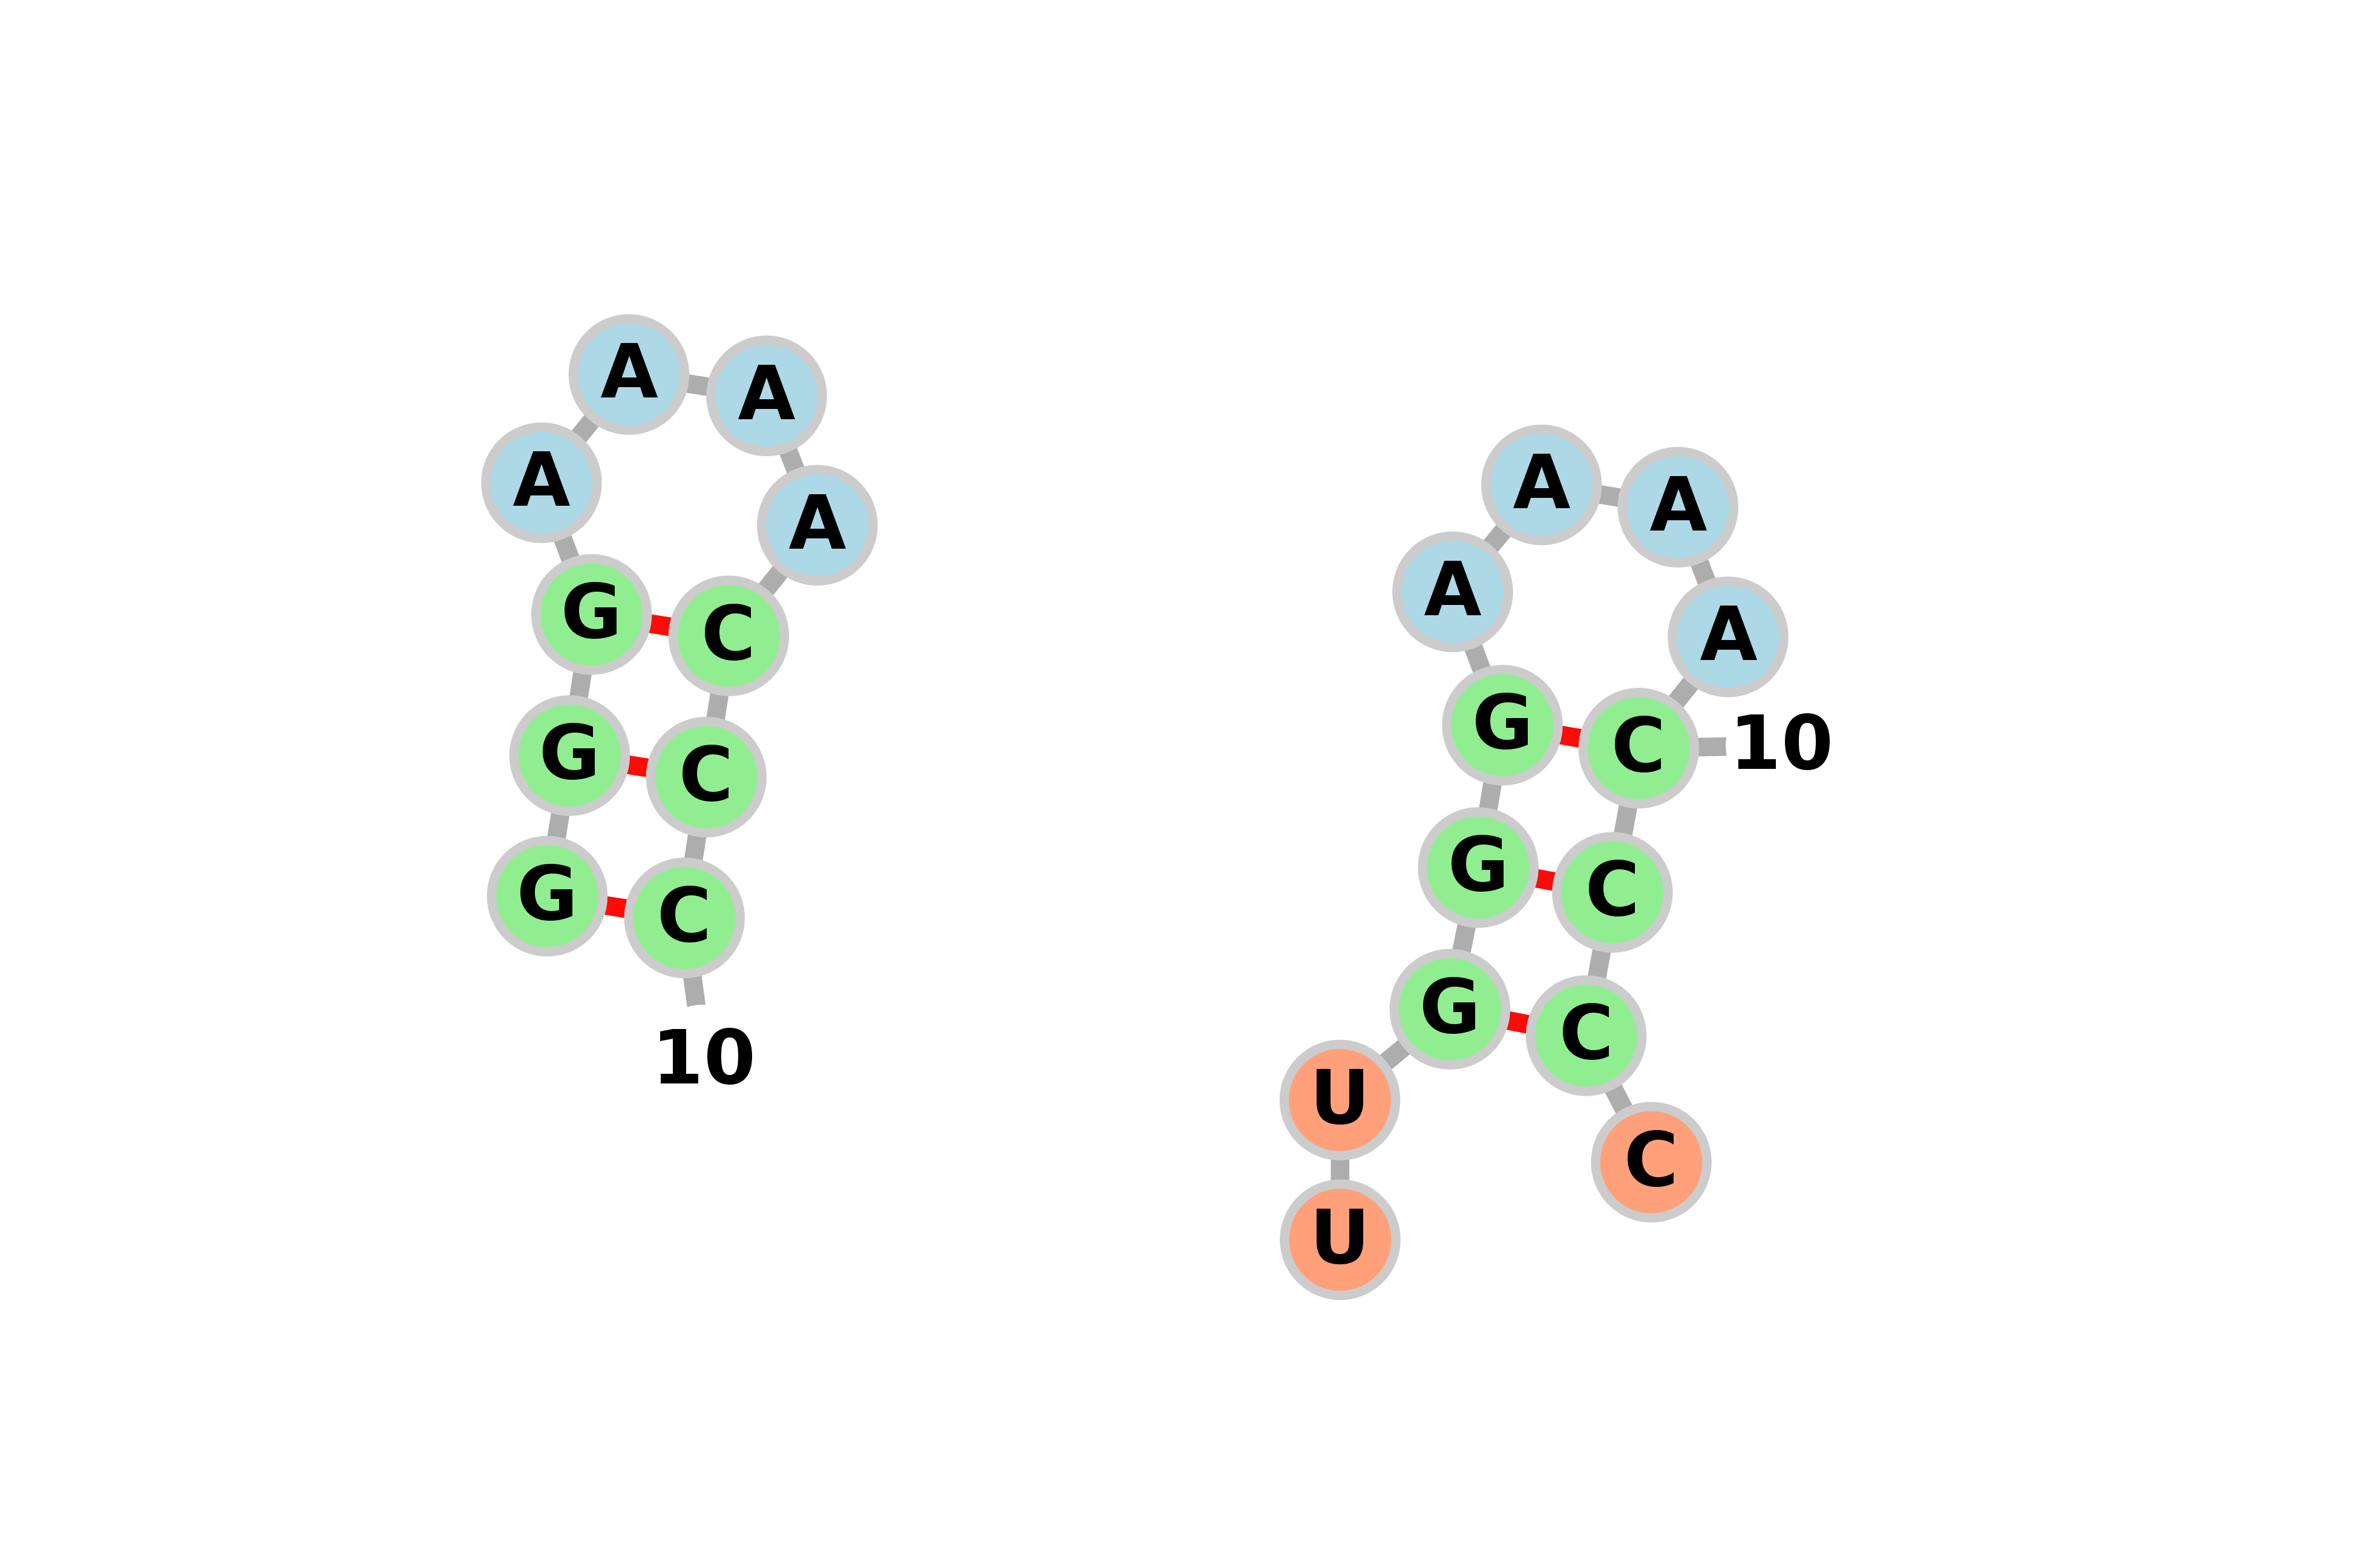
\includegraphics[width=0.4\textwidth]{./pictures/dangling.png}
	\label{fig:dangling}
\end{figure}
}

%Dangling is the effect of stacking an unpaired base to an adjacent helix. 
%Dangling is one of the highest energy contribution apart from the sugar-phosphate backbone and base-pairs and is significantly decreasing the free energy.
%2 dangle models are used within my thesis, Dangle 0 and dangle 2.


%I decided to spare you the exact details of the how the kinwalker algorithm is working, but if someone really is interested, I have backup slides and I can of course explain it.
%If not I'm just going to explain the output of a kinwalker run and the chosen parameters.
%
%I studied four parameters of the kinwalker algorithm. Transcription rate, the implemented pathfinding algorithm, the maxkeep parameter which defines the amount of simultaneously followed paths if a breath first search is chosen in the pathfinding algorithm and the dangle option which is similar to the choosen energy calculation model. 
%
%And on this picture we can also see a kinwalker outputfile.
%The first two lines define the RNA sequence, as well as the MFE structure of this RNA sequence. Each line also shows the free energy of this structure (here -60 kcal/mol, this is the MFE structure).
%The last structure in the output again, shows the MFE structure and the last line shows the whole runtime of the algorithm.
%In between, the whole folding trajectory is shown.
%Every line shows:
%(1) the current formed structure in dot bracket format, (2) the free energy
%of this specific structure, (3) overall passed time since the beginning of
%transcription, (4) the energy barrier to get from the previous structure to
%the current structure, (5) allowed max energy barrier, and (6) number of bases already transcribed.

% the last line is always the MFE structure, and here we can see a local energy minimum or folding trap

\frame{
\begin{figure}
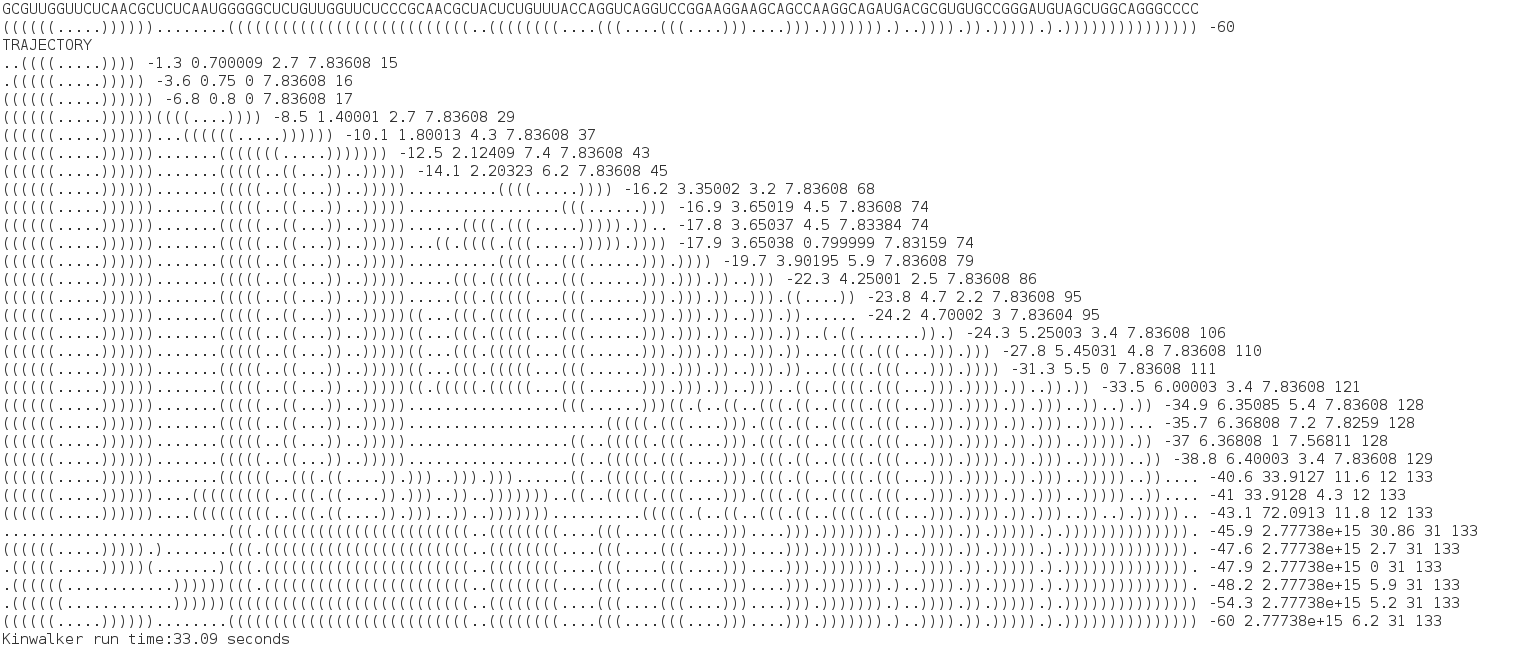
\includegraphics[scale=0.3]{pictures/KinwalkOutput.png}
\end{figure}

}


\frame{
\frametitle{RNA families used}
\begin{itemize}
\item \texttt{SRP}, \texttt{trpL}, \texttt{RNaseP}
\item 20-25 sequences per RNA family
\item from \texttt{RFAM database}
\end{itemize}

\begin{table}
\begin{tabular}{l|l}
ref. SRP functional structure & ref. SRP transient structure \\
\hline \\
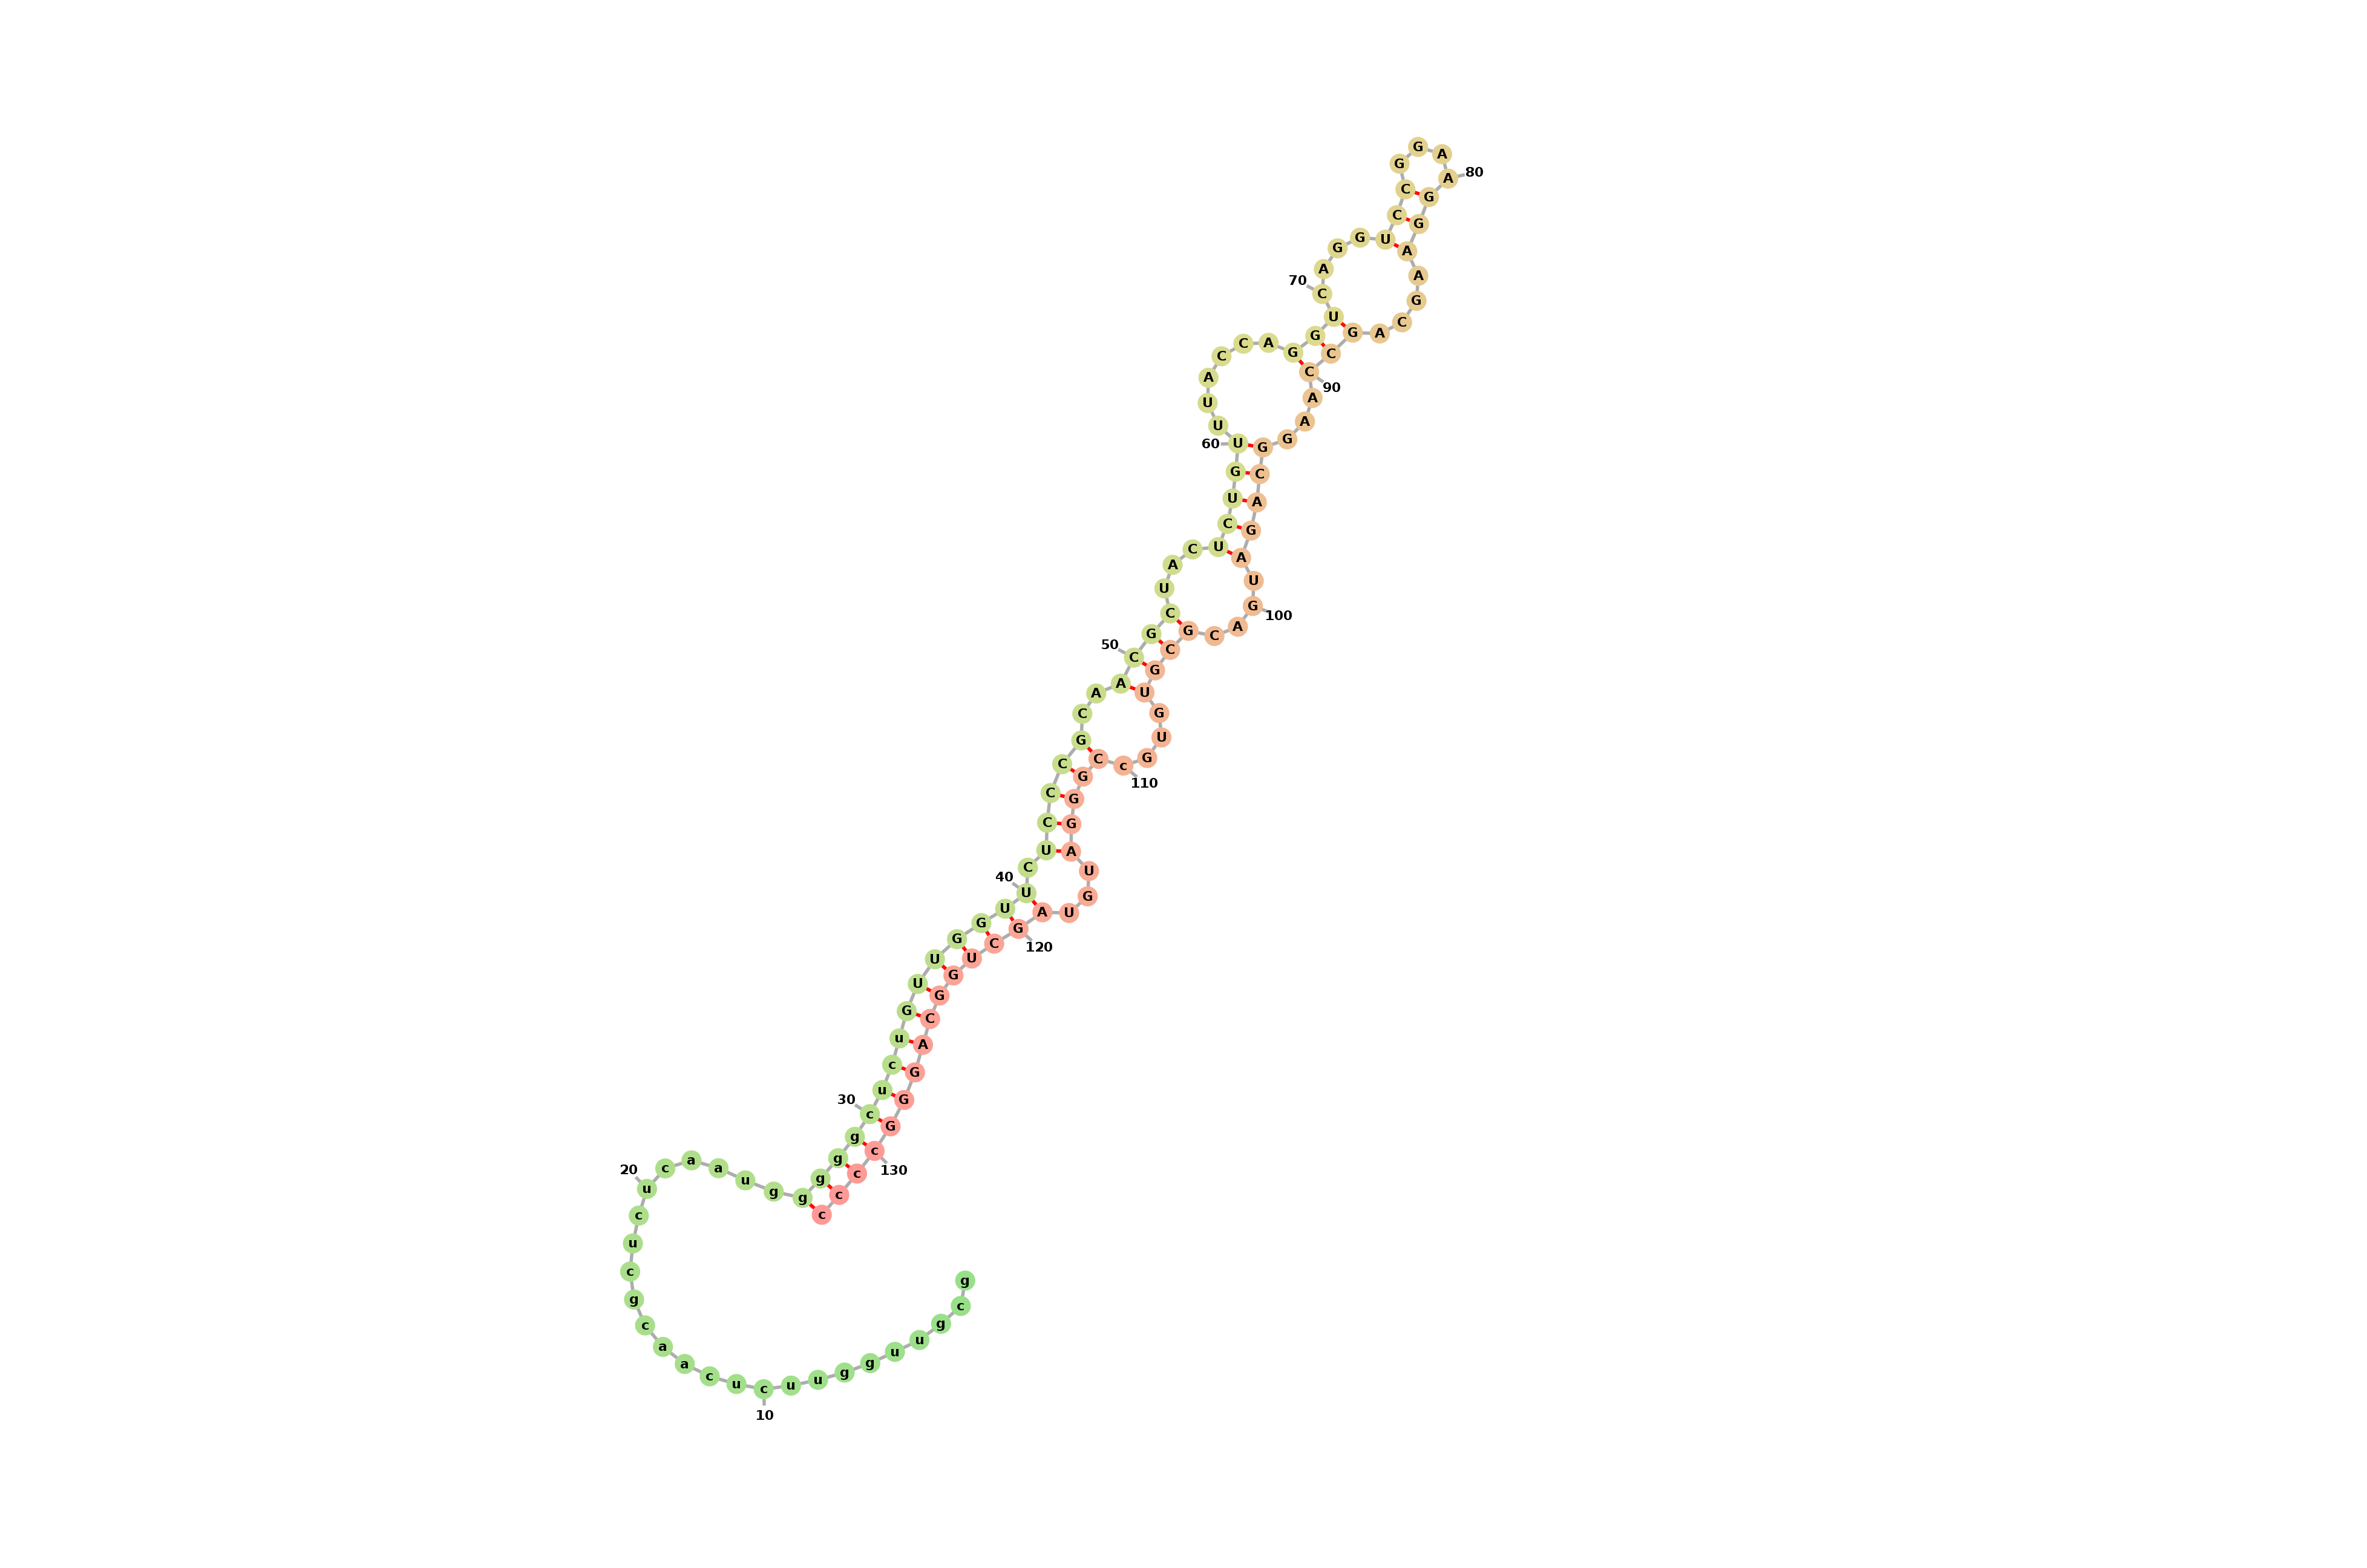
\includegraphics[width=0.5\textwidth]{./pictures/X01074-1-functional-str.png} &
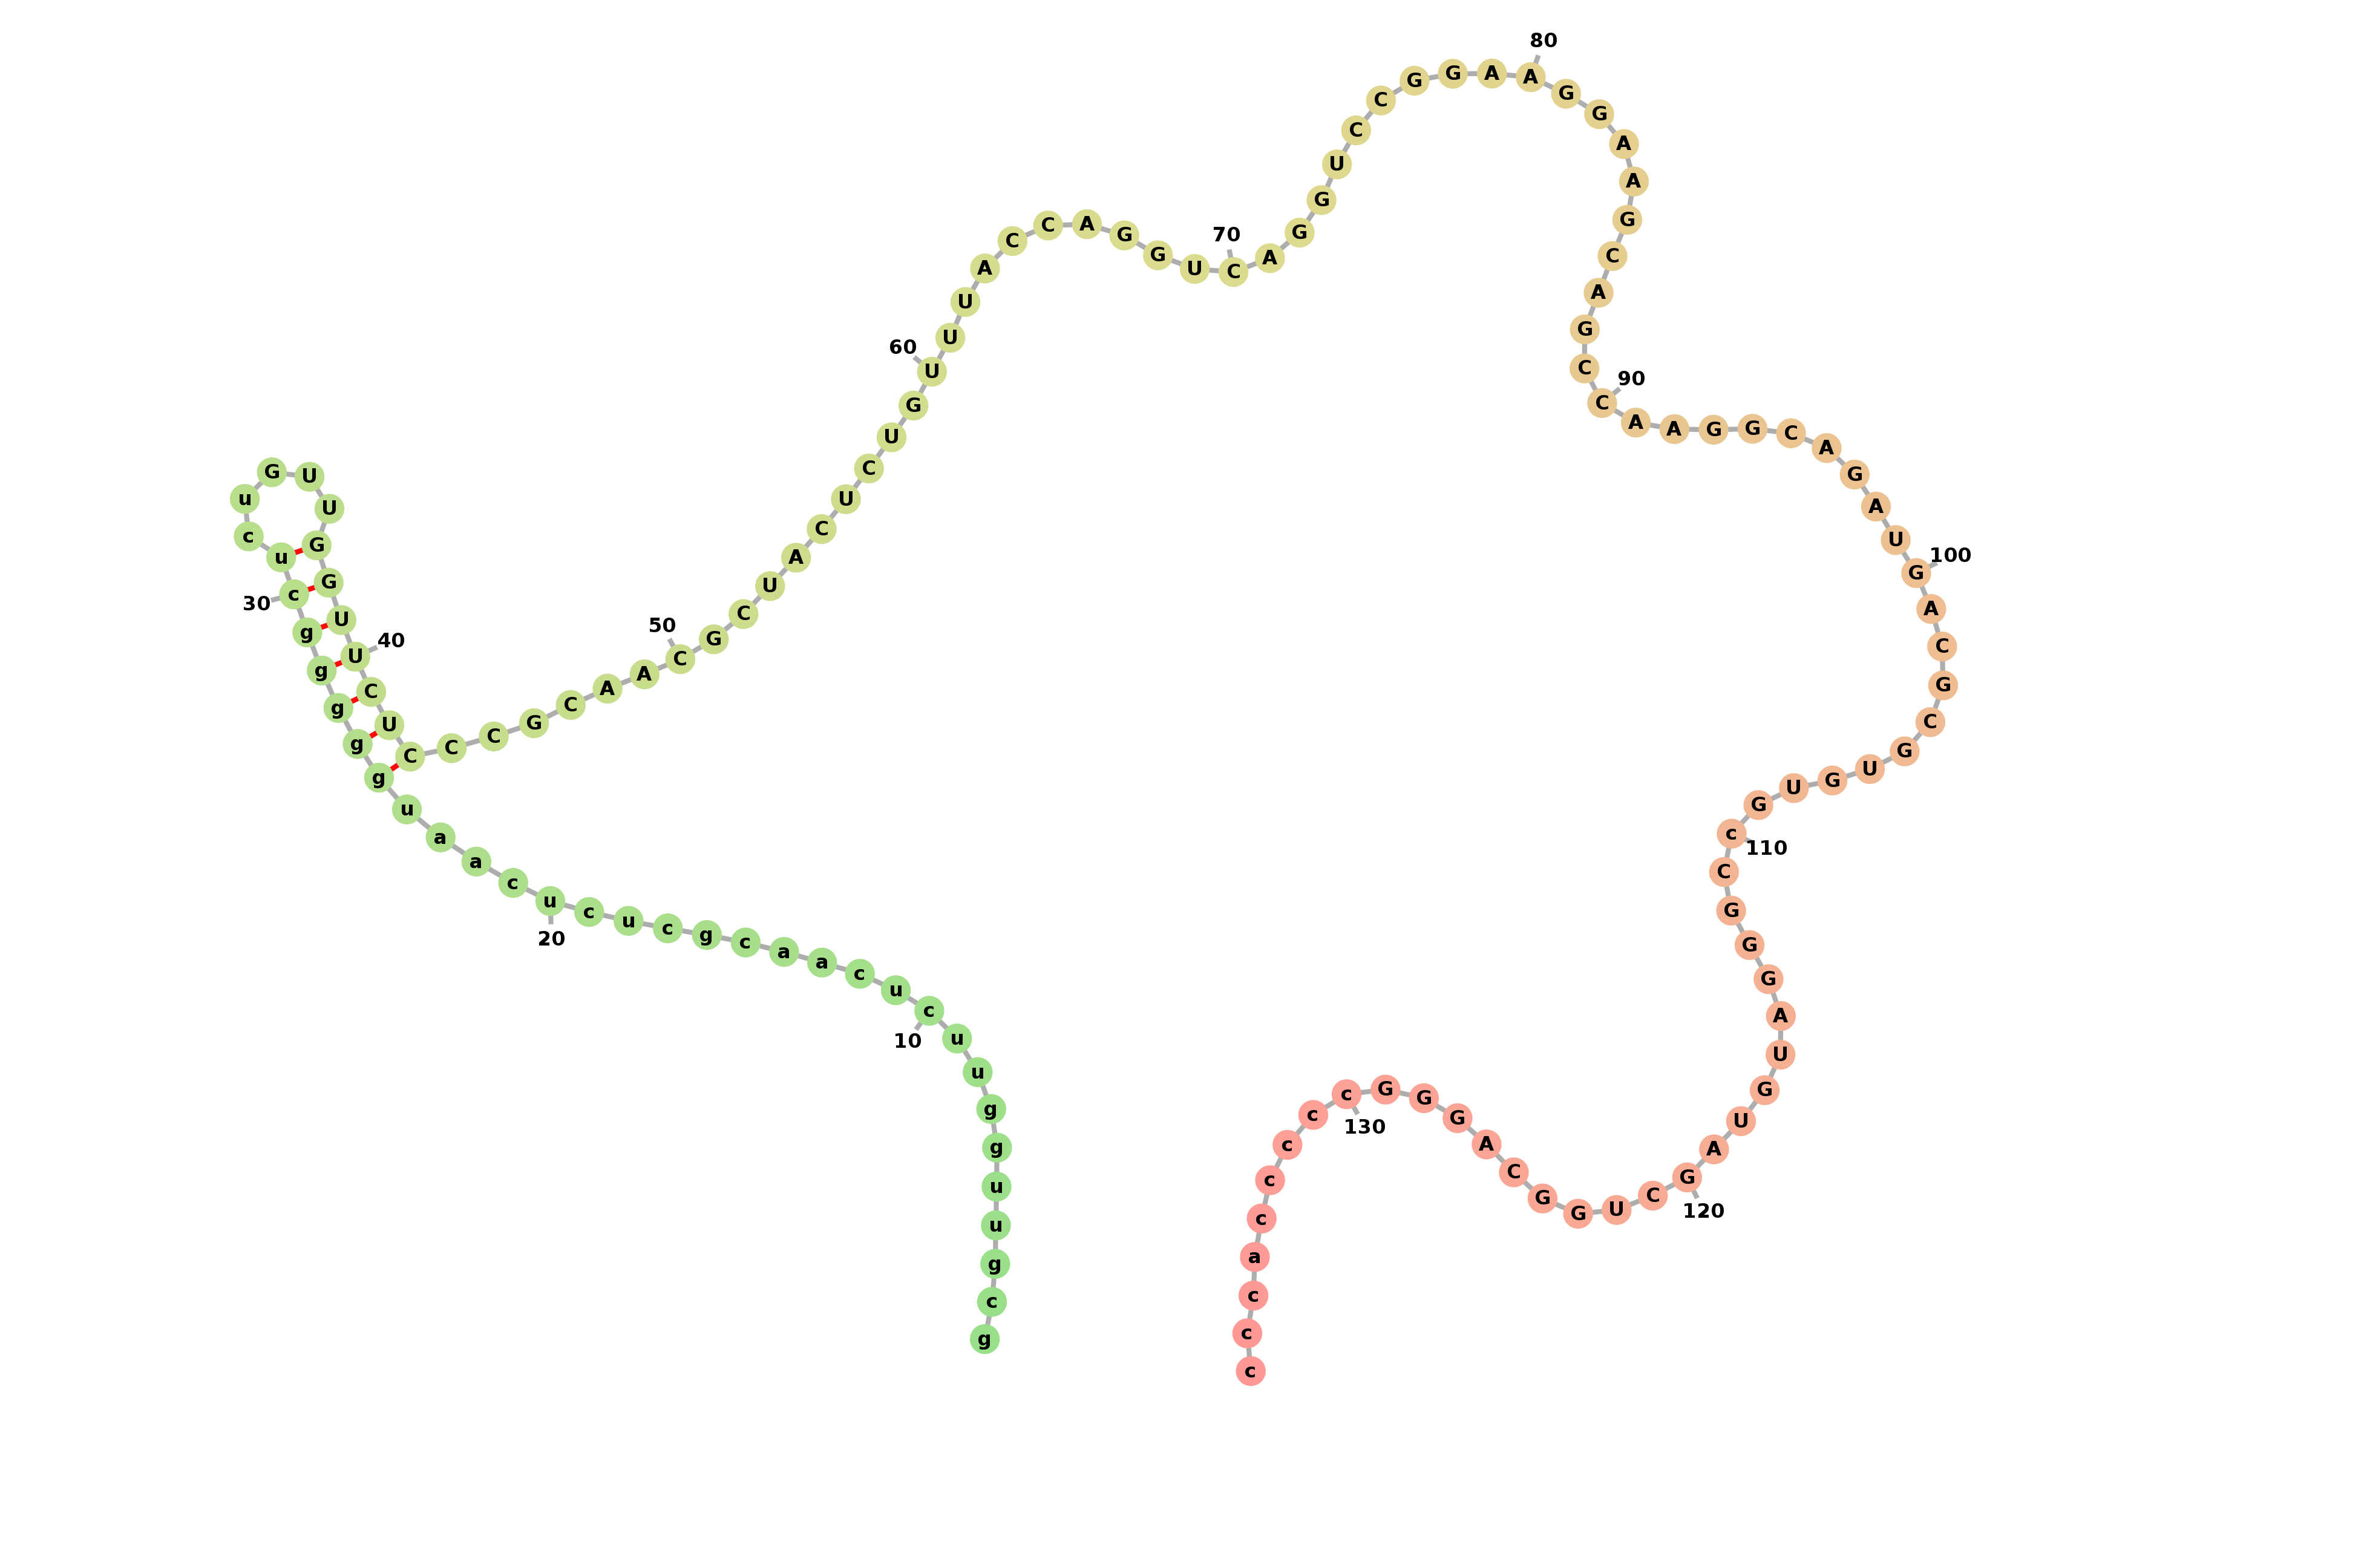
\includegraphics[width=0.5\textwidth]{./pictures/X01074-1-transient-str.png} \\
\end{tabular}
\end{table}
}

%I studies three different RNA families, each of them containing about 20-25 sequences. The first family is the RNA part of the signal recognition particle, the second one the tryptophan leader transcript and last the bacterial ribonuclease P.
%I chose this RNA families because they are already well studies, have existing benchmarking studies, there are reference sequences and refrence structures available and even co-transcriptional folding intermediates.
%Within this talk I am only going to show you the results of the SRP family, due to time limitations.
%The SRP reference sequence is able to form 2 different structures, the functional structure on the left and the transient structure on the right. Both of this structures were experimentally identified with cristallographic methods.


\frame{
\frametitle{SRP Sequence similarity \& structure conservation index}

\begin{table}
\begin{tabular}{l|l}
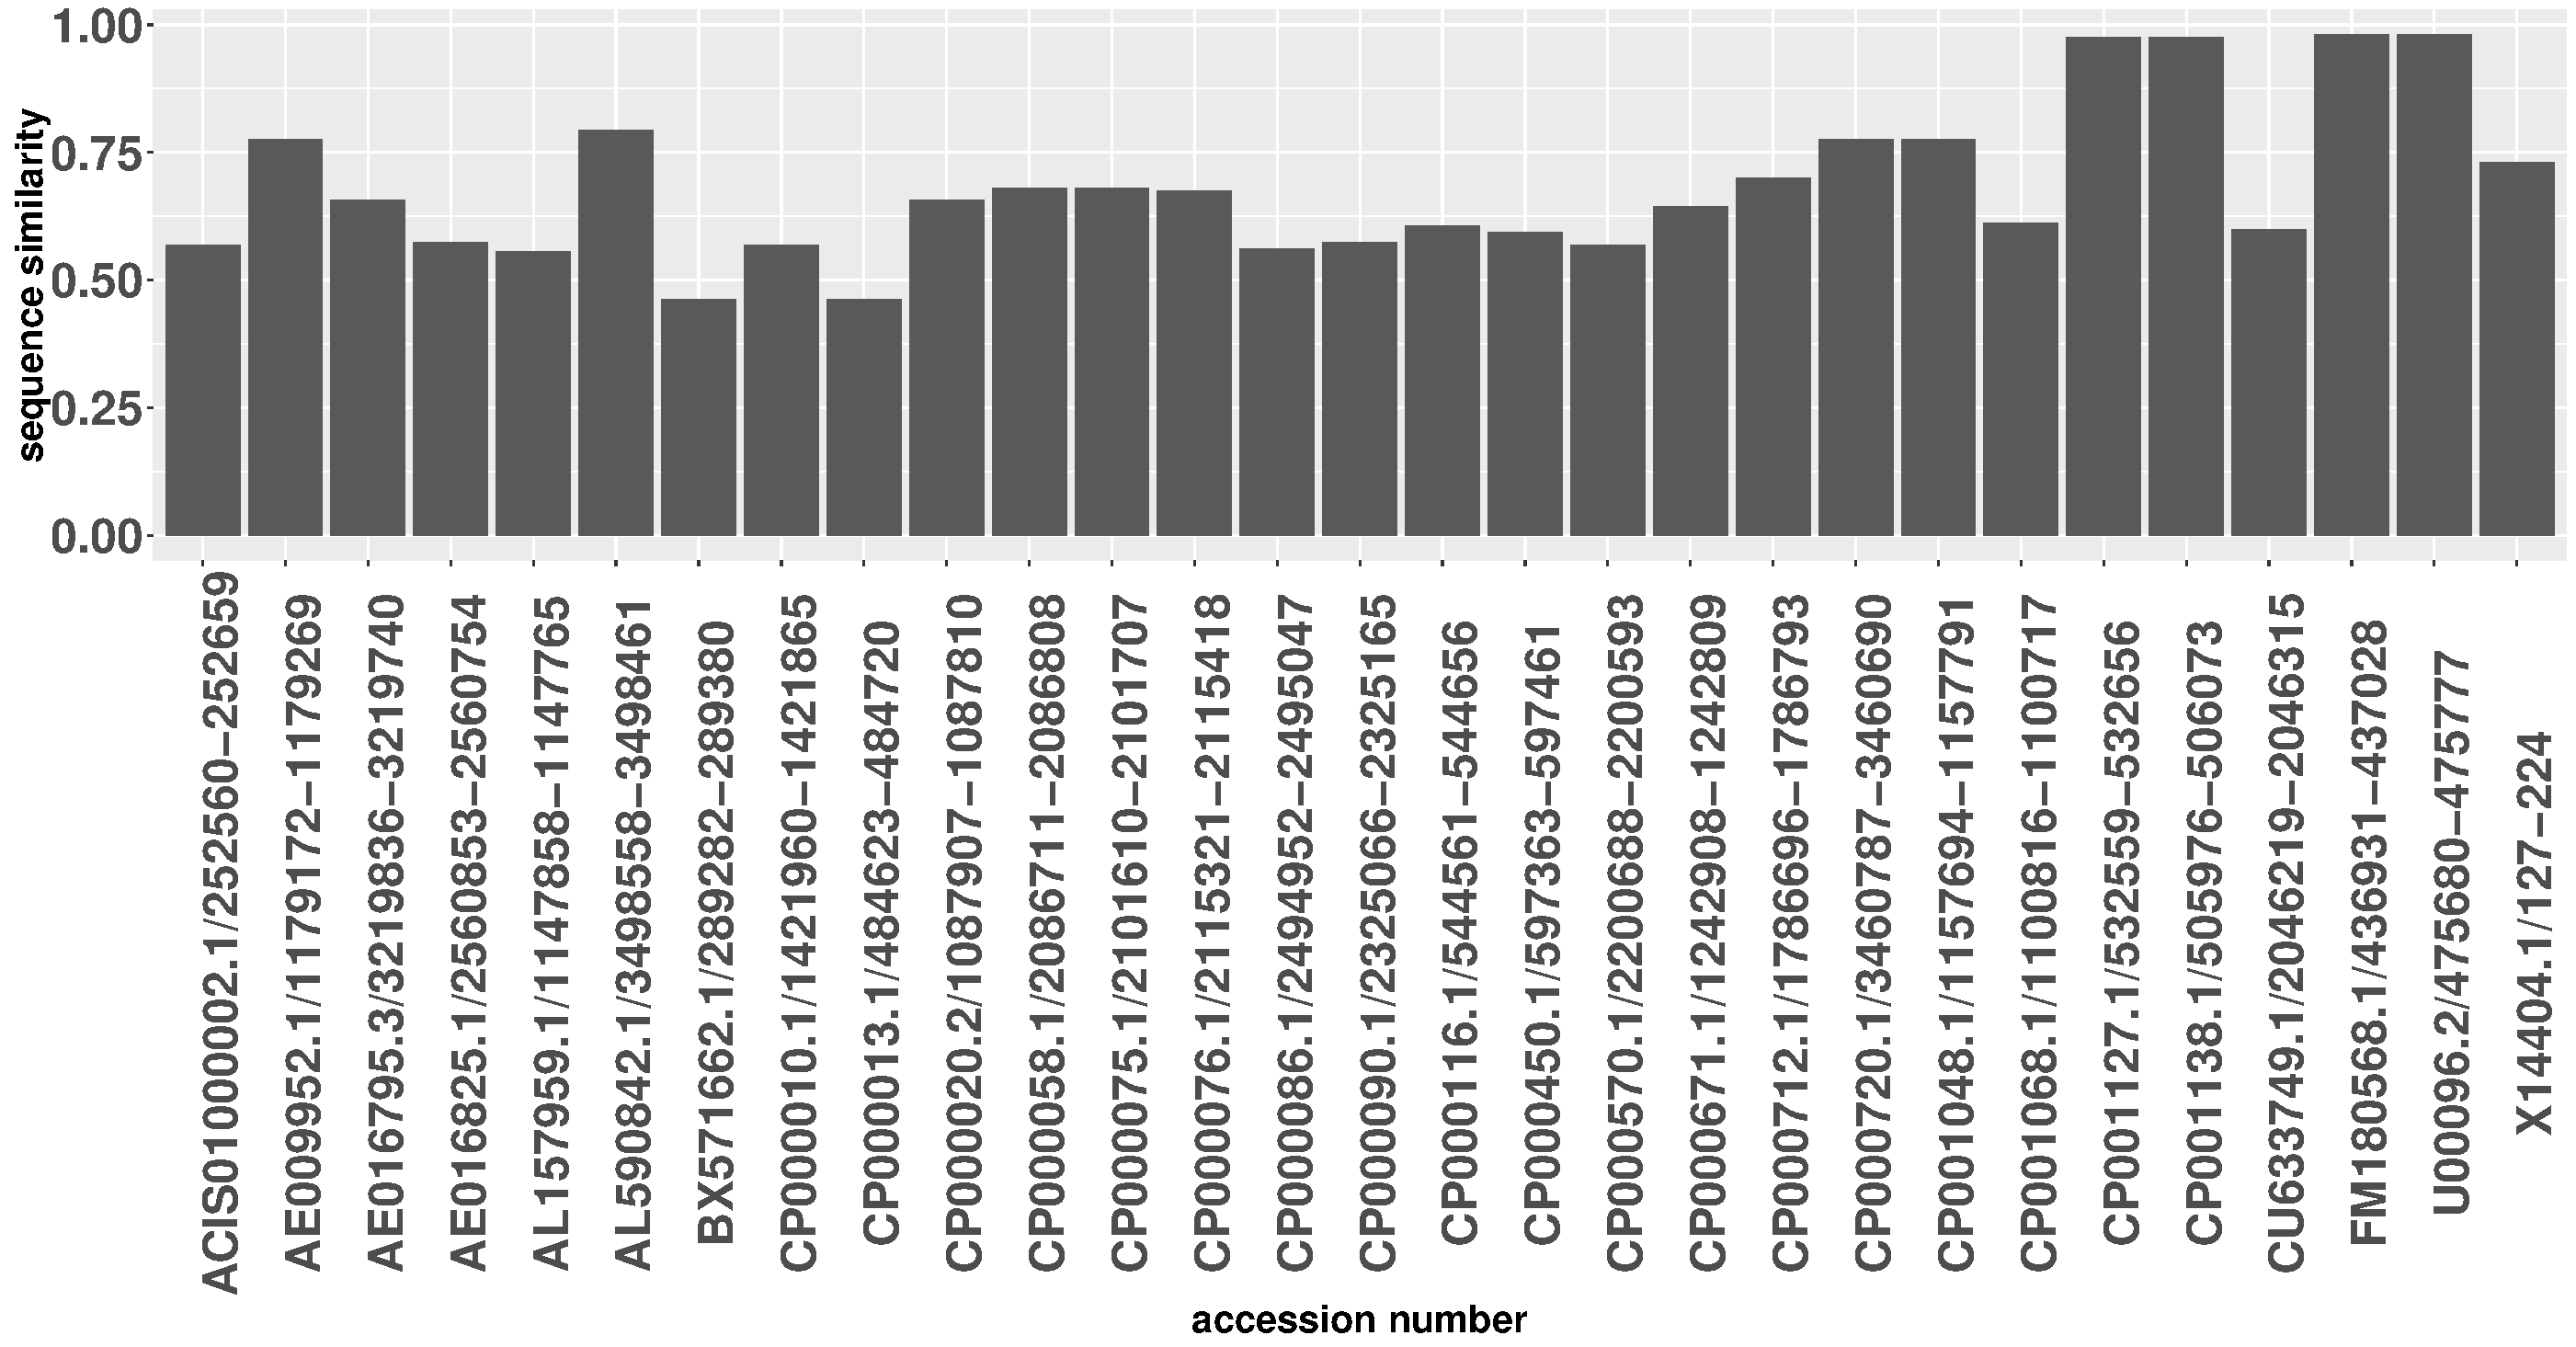
\includegraphics[width=0.5\textwidth]{./pictures/SS_SRP.pdf} &
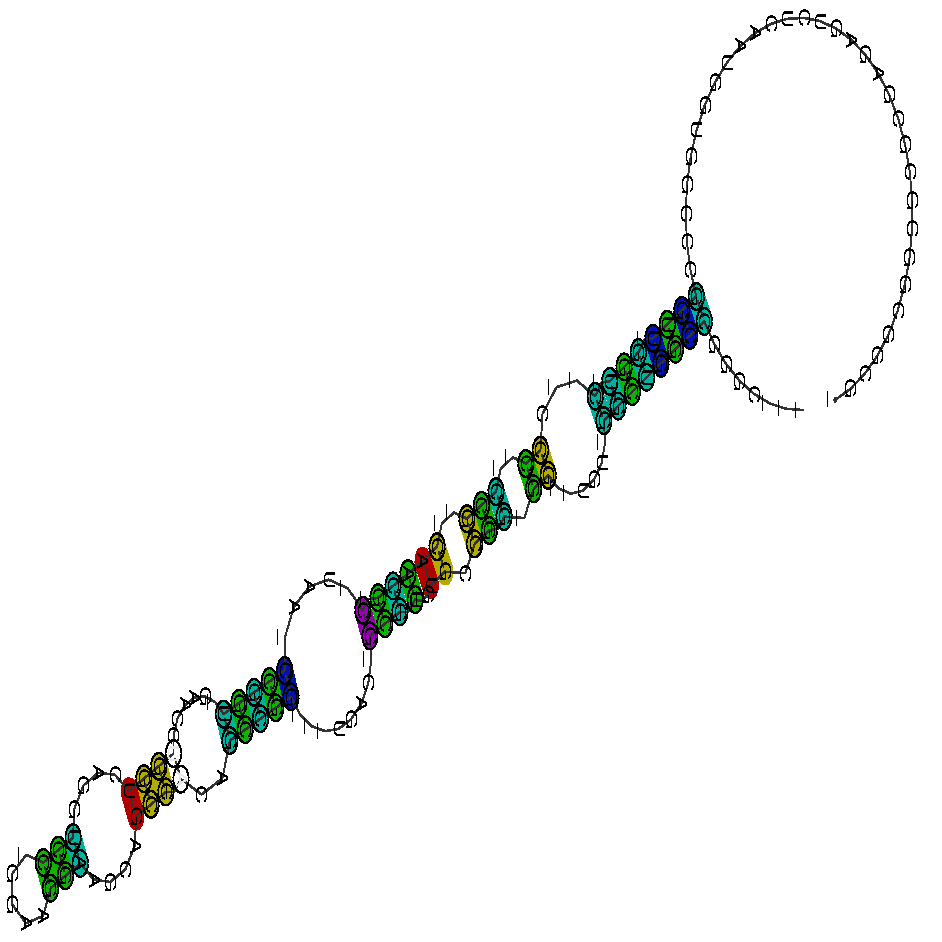
\includegraphics[width=0.4\textwidth]{./pictures/SCI_SRP.pdf}


\end{tabular}
\end{table}


\begin{equation}
SCI(A) = MFE(\mbox{consensus structure}) \cdot \frac{1}{\frac{1}{|A|}\cdot \sum\limits_{a\in A} MFE(a)}
\end{equation}

}


%Finally I can show you some results and like I said I focus primarely on the SRP family, but I calculated many different scores to analyze the kinwalker results with different parameters and different RNA families.
%Describe the figure!!!


\frame{
\frametitle{Ensemble diversity of SRP reference sequence}
\begin{figure}
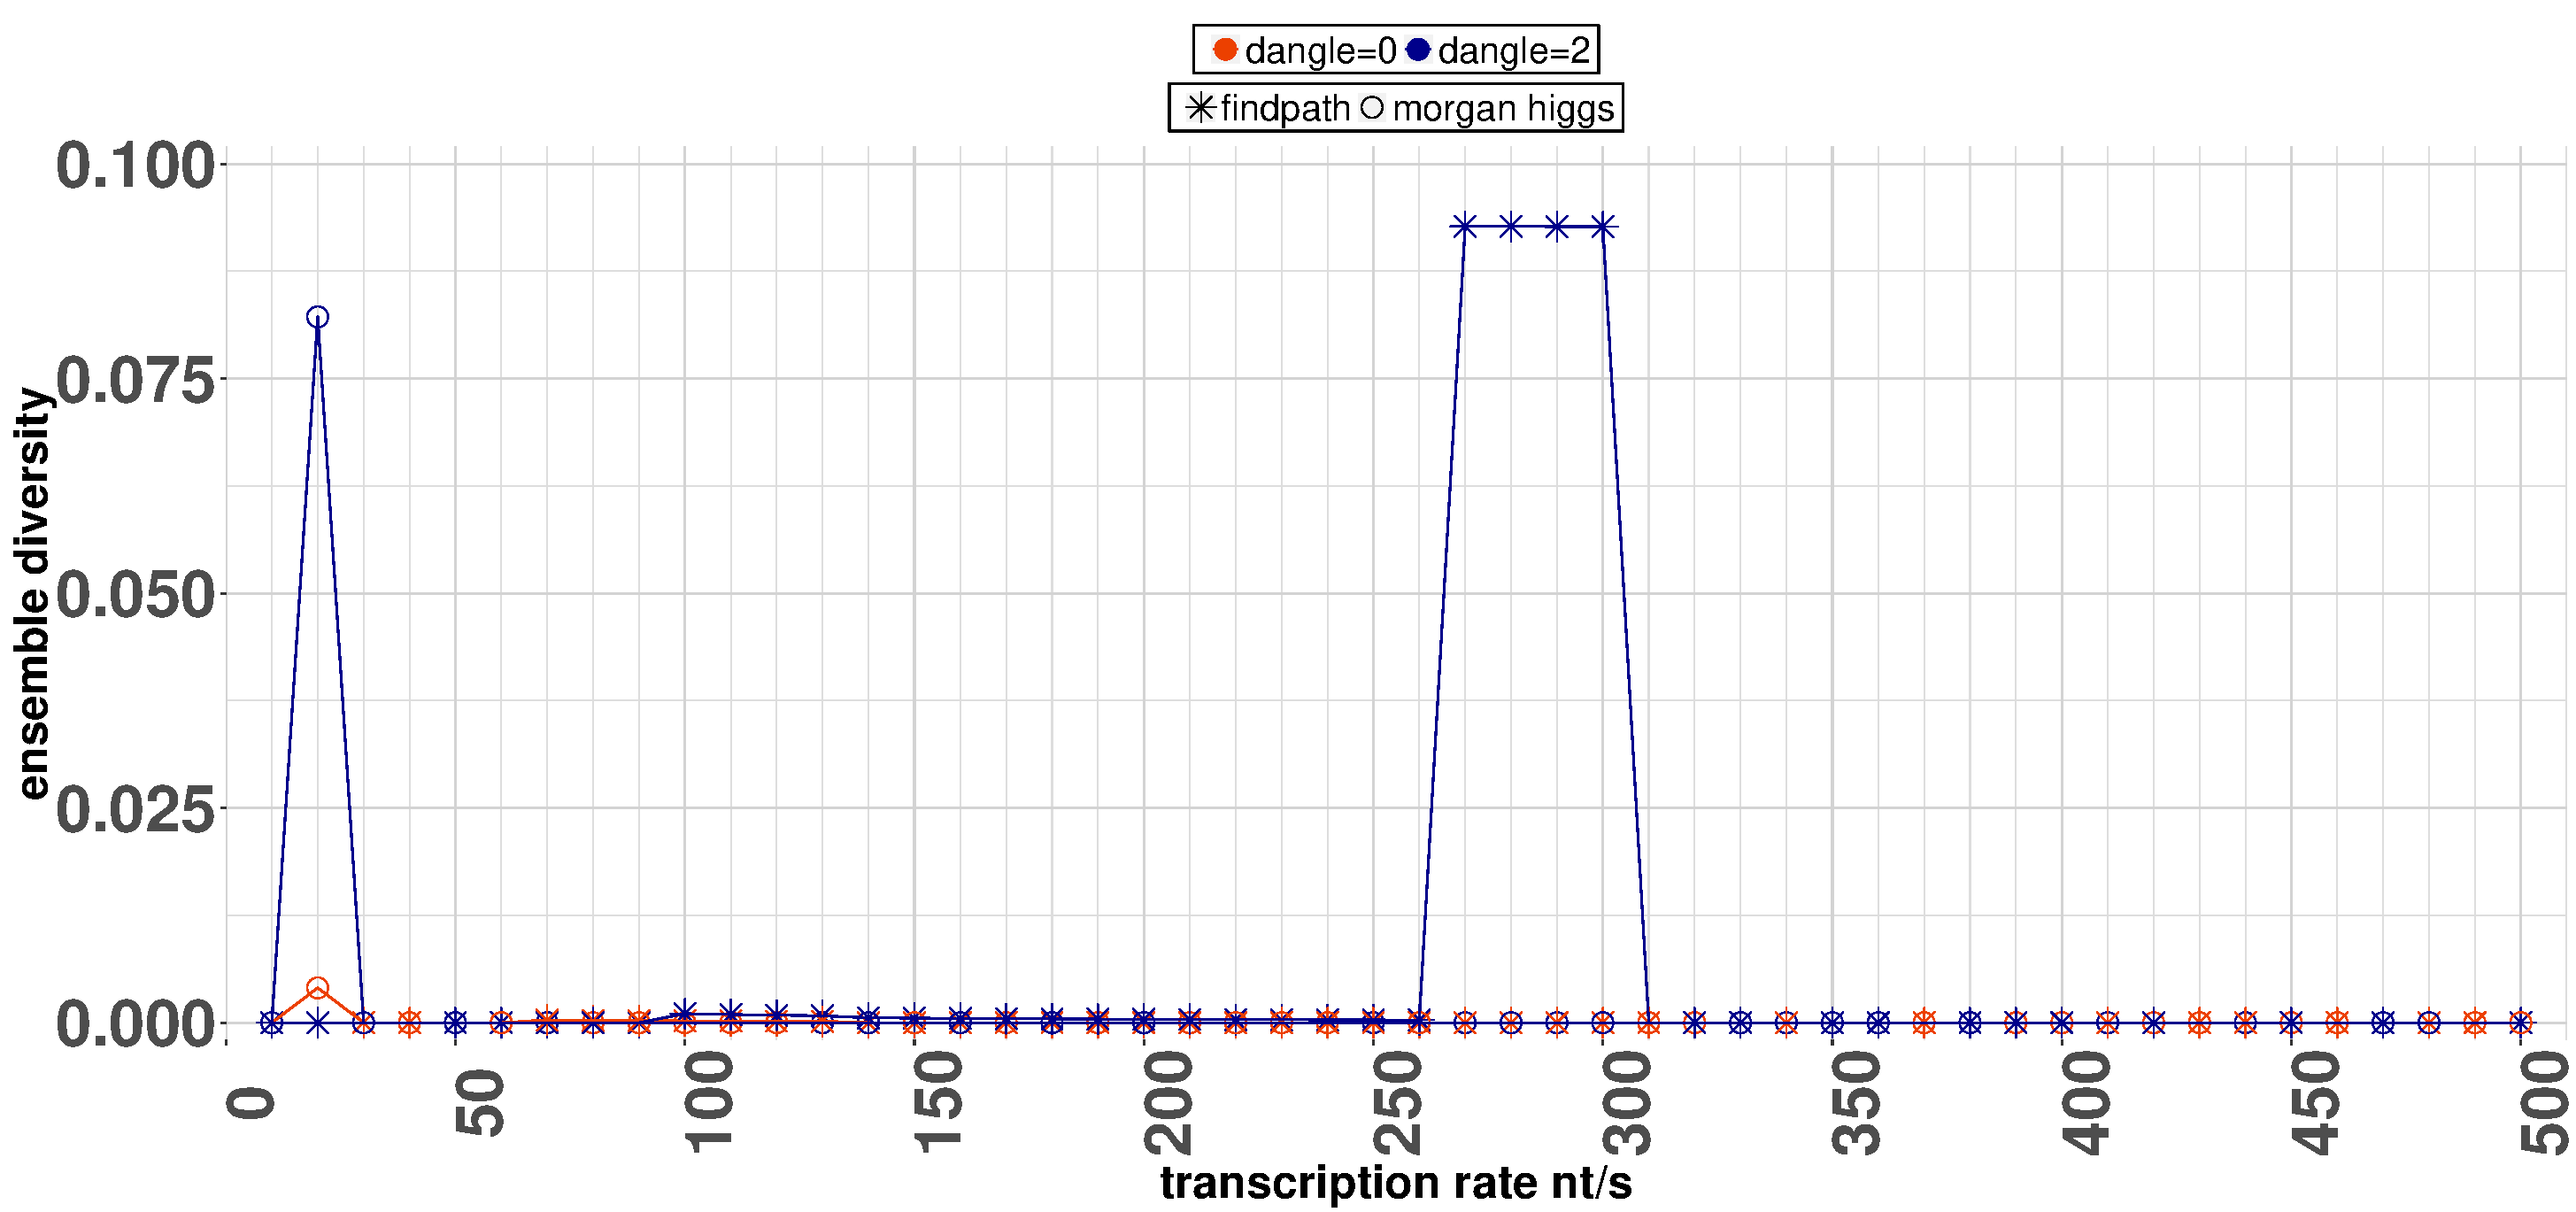
\includegraphics[scale=0.2]{pictures/SRP2510.pdf}
\end{figure}

\begin{equation}
\begin{cases}
\mbox{ensemble diversity} = \frac{1}{l} \cdot \sum\limits_{i,j} (p(i,j))\cdot (1- p(i,j))  \\
p(i,j) =\frac{\Delta Time_{ij}}{period}
\end{cases}
\label{eq:ensemble diversity }
\end{equation}



}

%


%I analyzed the corresponding kinwalker output data files for this region and came to following conclusion. 
%In this area the SRP reference sequence folds relatively early into
%the MFE structure. During he first half of transcription, it creates non MFE base-pairs at the 5' end similar to the ones experimentally identified as transient structure. These transient hairpins seem to prevent the sequence from forming stable intermediate structures and thus falling into a folding trap.
%
%And with every other parameter combination, the sequence
%falls into a folding trap. The predicted time needed to refold into the MFE structure precedes the life-time of an RNA molecule, and is
%therefore only theoretically possible.
%
%That means that I found the correct paramter combination to predict co-transcriptional folding of the SRP reference sequence.
%


\frame{
\frametitle{backup slides}

}
\frame{
\frametitle{Ensemble distance of SRP family to SRP transient}

\begin{figure}

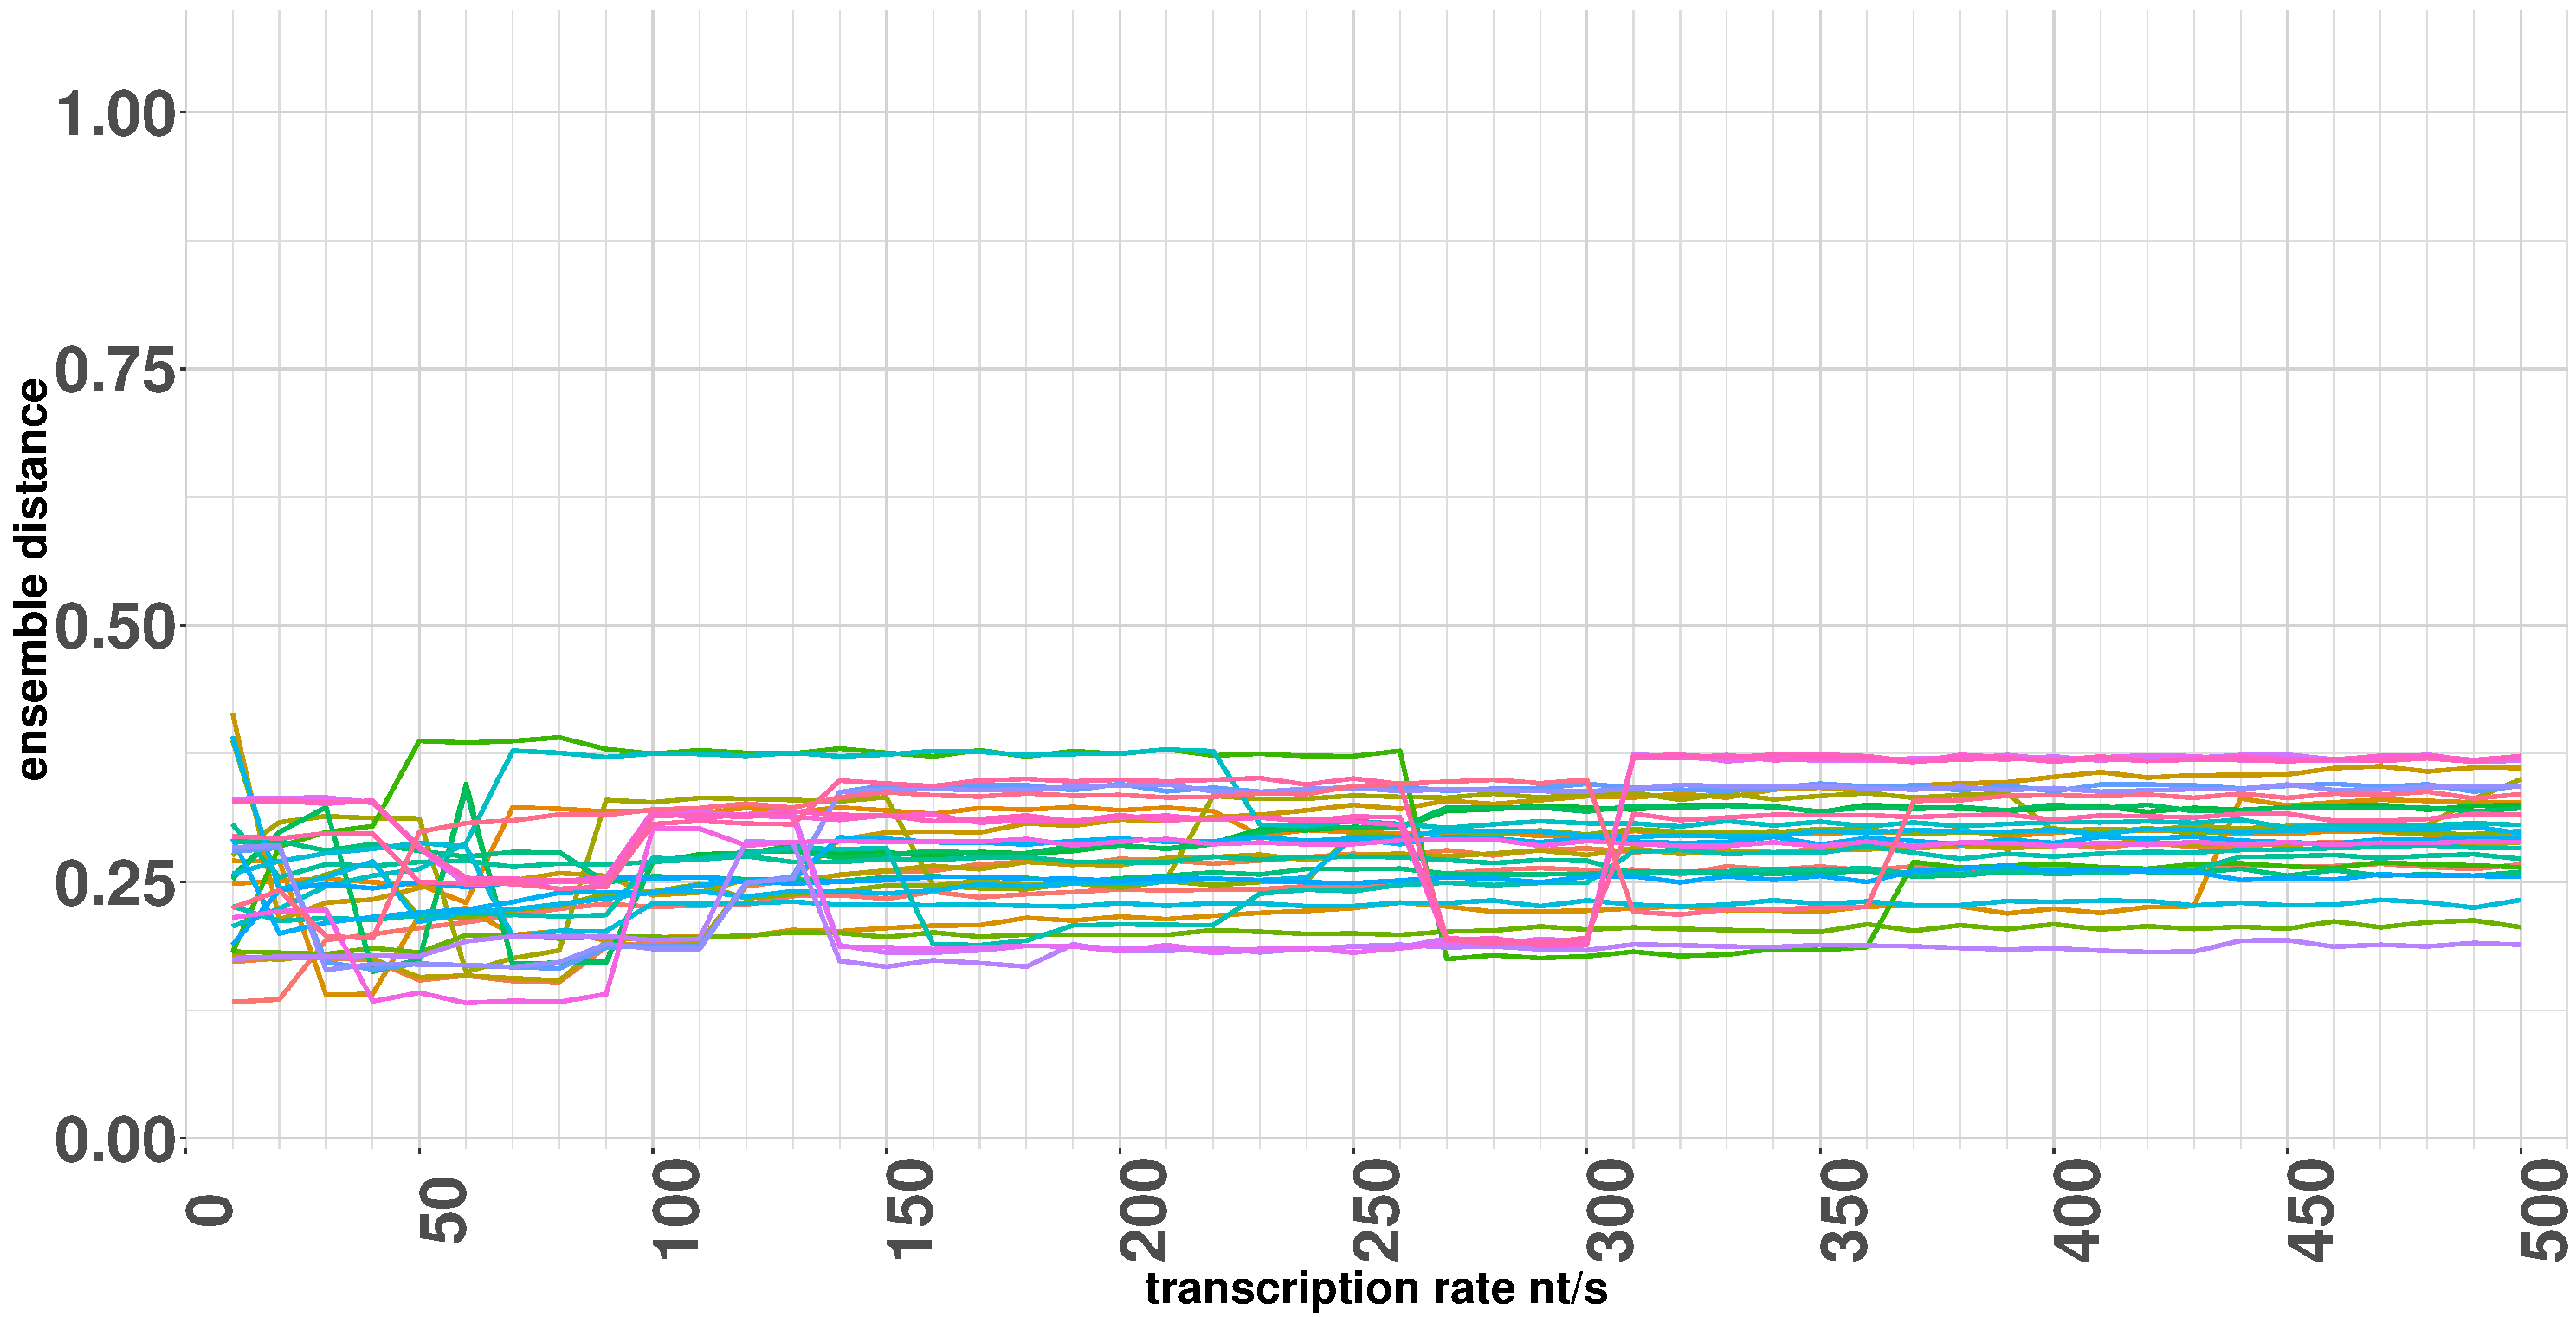
\includegraphics[width=0.9\textwidth]{pictures/ensembleDistance_SRPtransient.pdf}\\
\end{figure}

\begin{equation}
d_{E,T}(M,s_{ref})= \sum\limits_{(i,j)_M \in s_{ref} } (1- p(i,j)) + \sum\limits_{(i,j)_M \notin s_{ref}} p(i,j),
\label{eq:ensemble distance}
\end{equation}



}





\frame{
\frametitle{consensus structure}

}


\frame{
\begin{figure}
\begin{tabular}{l}
 REALLY want to introduce bp diversity here!!!!
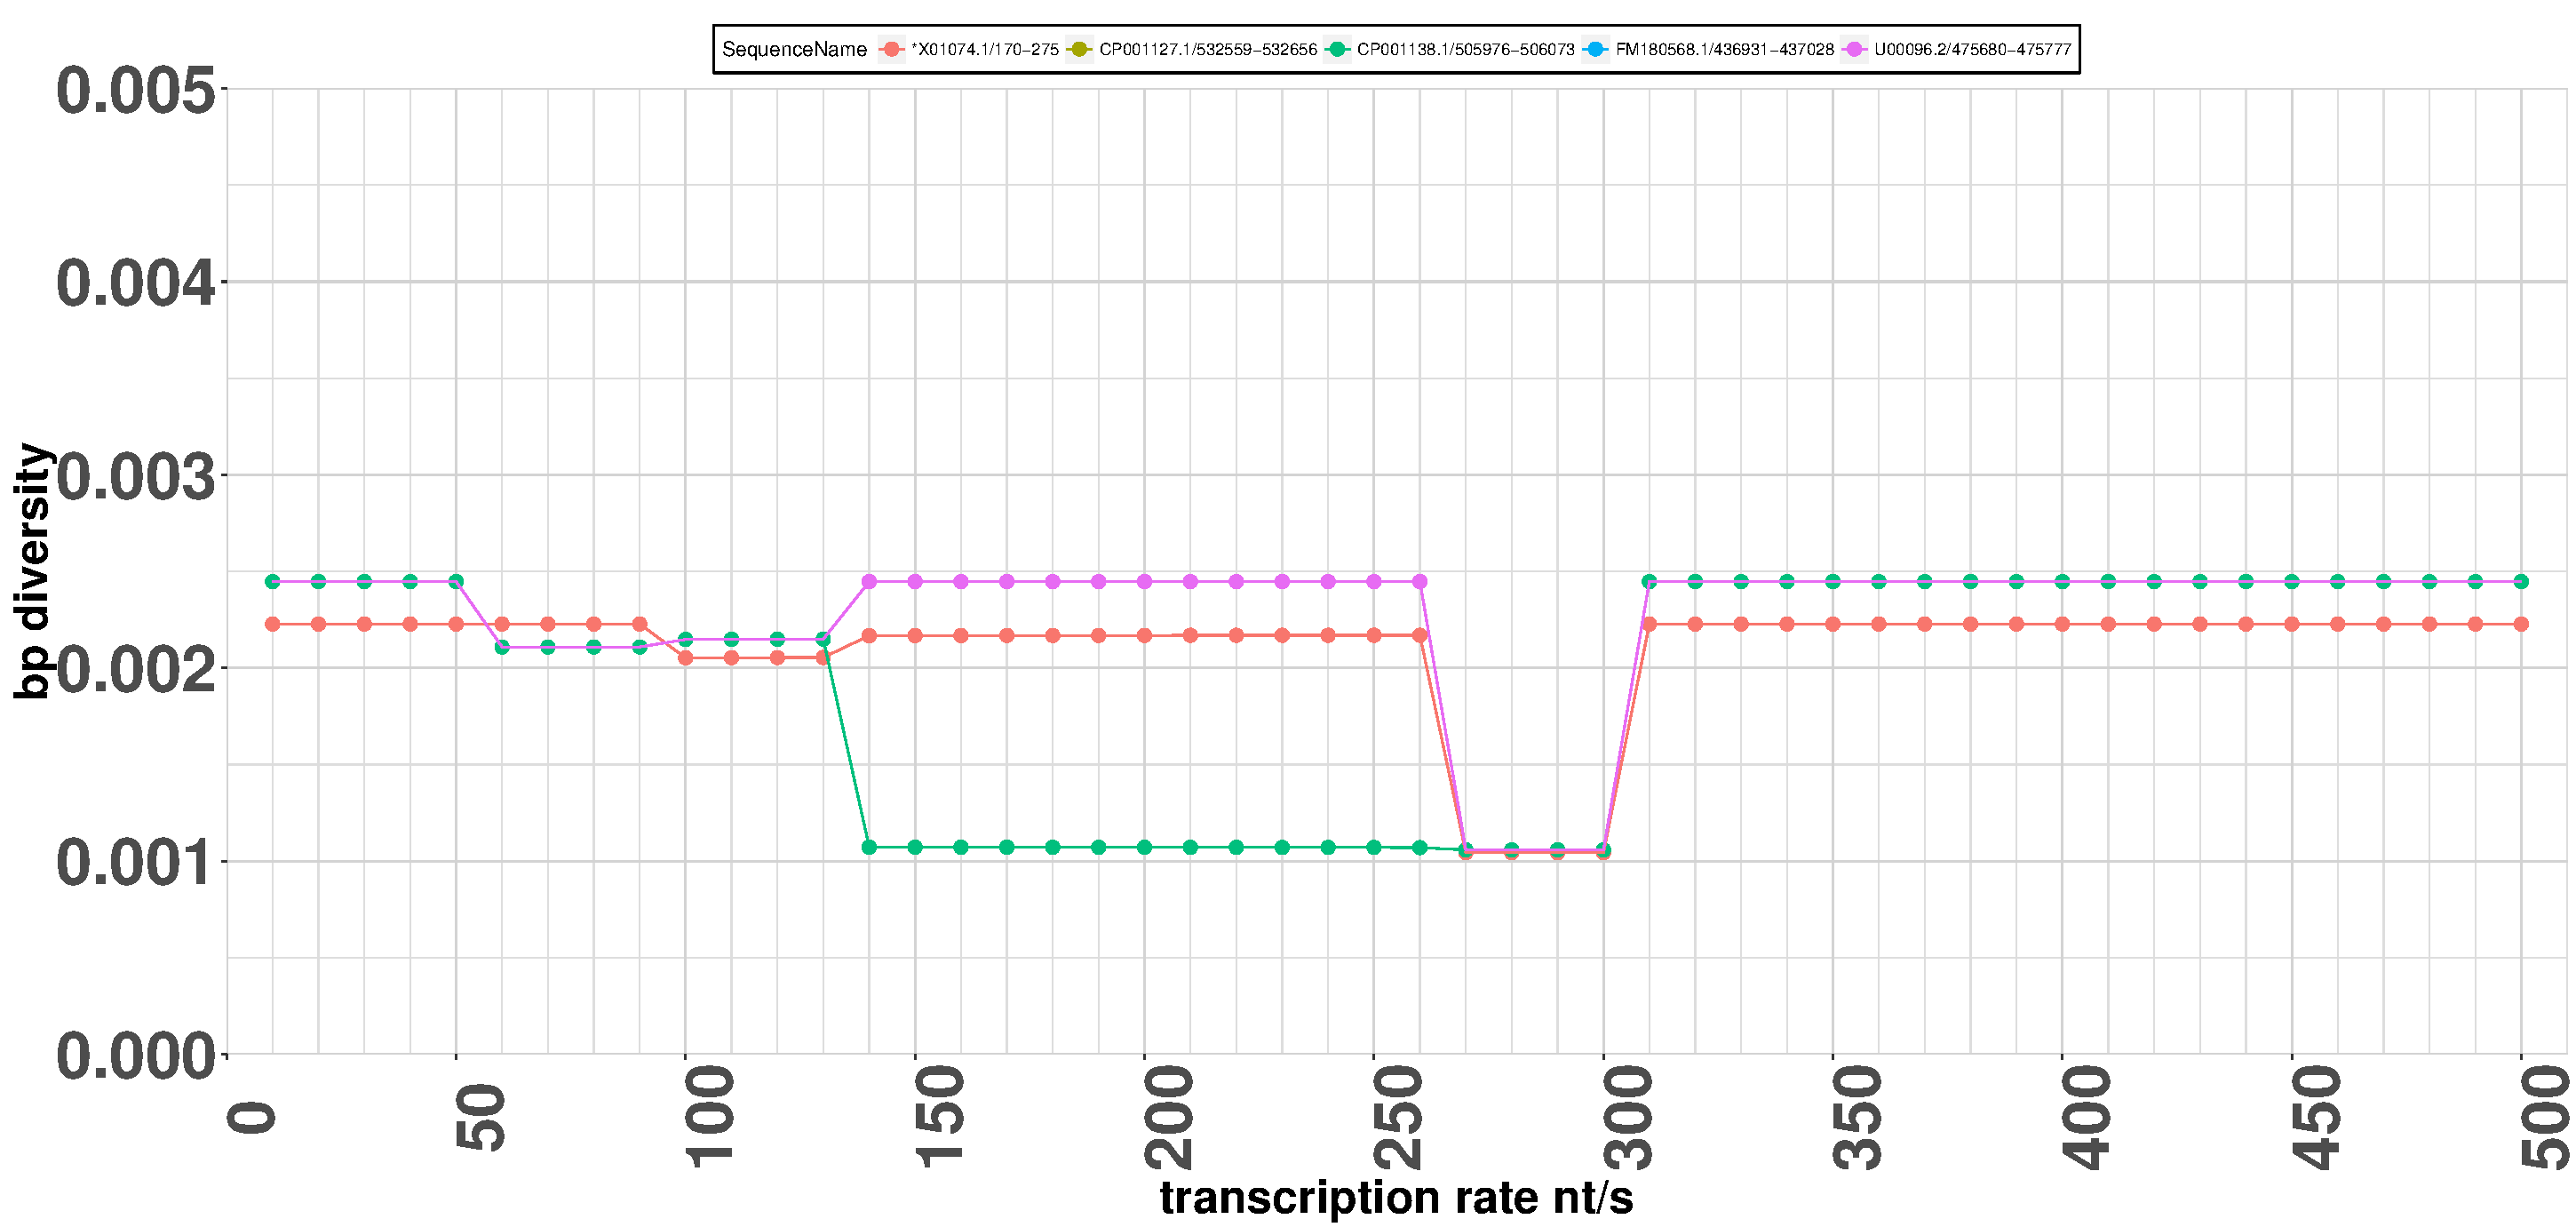
\includegraphics[width=1.0\textwidth]{./pictures/SRPseqDecrease250_300nts.pdf}\\

\end{tabular}
\end{figure}

}






\end{document}

